\section{Experiments}
\label{sec:exp}
We evaluate TurnOPD on three representative agent tasks: ALFWorld (embodied text planning), Multi-Hop Search, and WebShop (web navigation), using three different student-teacher pairs that span multiple model sizes and model families. 
We test whether TurnOPD achieves a better accuracy--time frontier across different environments and models.

\textbf{Students and teachers.} 
Students are distilled from stronger, task-specialized GRPO-trained teachers: ALFWorld uses Qwen3-1.7B/4B students with a Qwen3-8B-GRPO teacher; WebShop uses Qwen3-1.7B and Qwen3-8B-GRPO; Multi-Hop Search uses Qwen3.5-2B and Qwen3.5-9B-GRPO. All methods use the same OPD reverse-KL training stack.

\textbf{Baselines and Metrics.} We evaluate three primary methods: vanilla OPD, TCOD-F2B~\citep{wang2026tcod}, and TurnOPD. To ensure a fair and comprehensive comparison, we conduct evaluations under two regimes: \textit{Least-Time}—where we compare all methods based on accuracies achieved at the minimal wall-clock time required for any method to reach 100 training steps; and \textit{Same-Step}—where each method is evaluated after exactly 100 training steps. Accuracy for each method is reported as the average accuracy over the last four evaluation points (each point is calculated using Avg@4) before the corresponding cutoff. We also report the standard deviation of the accuracy over the last four evaluation points.
In addition, we include the performance of the GRPO-trained teacher models as reference points. Note that teacher accuracy is intended for context and not as a baseline for efficiency comparisons.


% \begin{table*}[tbp]
%     \centering
%     \caption{Main comparison across 3 tasks with per-sub-benchmark breakdown. The best results are in bold. ``sub-bench'' denotes the sub-task or category within each benchmark. The accuracy is reported as the avg@4 before the corresponding cutoff. Aggregated metrics are to the right.}
%     \label{tab:main}
%     \scriptsize
%     \setlength{\tabcolsep}{3.2pt}
%     \resizebox{\textwidth}{!}{%
%     \begin{tabular}{@{}ll l l cccccc@{}}
%     \toprule
%     \textbf{Task}
%     & \textbf{Student}
%     & \textbf{Method}
%     & \textbf{sub-bench}
%     & \makecell[c]{\textbf{Acc by Category}\\\textbf{Least-Time}}
%     & \makecell[c]{\textbf{Overall Avg@4}\\\textbf{Least-Time}}
%     & \makecell[c]{\textbf{Overall Avg@4}\\\textbf{Same-Step}}
%     & \makecell[c]{\textbf{Wall}\\\textbf{(h)}}
%     & \textbf{Speedup} \\
%     \midrule
%     % ALFWorld Qwen3-1.7B
%     \multirow{30}{*}{ALFWorld} & \multirow{30}{*}{Qwen3-1.7B}
%       & \multirow{6}{*}{Zero-Shot}
%         & sub-bench 1 & 0.00 & \multirow{6}{*}{0.00} & \multirow{6}{*}{0.00} & \multirow{6}{*}{--} & \multirow{6}{*}{--} \\
%       &  &  & sub-bench 2 & 0.00 &  & & & \\
%       &  &  & sub-bench 3 & 0.00 &  & & & \\
%       &  &  & sub-bench 4 & 0.00 &  & & & \\
%       &  &  & sub-bench 5 & 0.00 &  & & & \\
%       &  &  & sub-bench 6 & 0.00 &  & & & \\
%     \cmidrule(l){3-9}
%       &  & \multirow{6}{*}{Teacher}
%         & sub-bench 1 & 92.50 & \multirow{6}{*}{90.75} & \multirow{6}{*}{90.75} & \multirow{6}{*}{--} & \multirow{6}{*}{--} \\
%       &  &  & sub-bench 2 & 93.40 &  & & & \\
%       &  &  & sub-bench 3 & 84.09 &  & & & \\
%       &  &  & sub-bench 4 & 92.34 &  & & & \\
%       &  &  & sub-bench 5 & 91.49 &  & & & \\
%       &  &  & sub-bench 6 & 91.28 &  & & & \\
%     \cmidrule(l){3-9}
%       &  & \multirow{6}{*}{Vanilla OPD}
%         & sub-bench 1 & 76.41 & \multirow{6}{*}{73.52} & \multirow{6}{*}{83.00} & \multirow{6}{*}{4.42} & \multirow{6}{*}{1.00$\times$} \\
%       &  &  & sub-bench 2 & 73.82 &  & & & \\
%       &  &  & sub-bench 3 & 65.45 &  & & & \\
%       &  &  & sub-bench 4 & 73.39 &  & & & \\
%       &  &  & sub-bench 5 & 75.93 &  & & & \\
%       &  &  & sub-bench 6 & 78.34 &  & & & \\
%     \cmidrule(l){3-9}
%       &  & \multirow{6}{*}{TCOD-F2B}
%         & sub-bench 1 & 82.66 & \multirow{6}{*}{80.06} & \multirow{6}{*}{80.06} & \multirow{6}{*}{\textbf{1.87}} & \multirow{6}{*}{\textbf{2.37$\times$}} \\
%       &  &  & sub-bench 2 & 80.19 &  & & & \\
%       &  &  & sub-bench 3 & 74.43 &  & & & \\
%       &  &  & sub-bench 4 & 79.03 &  & & & \\
%       &  &  & sub-bench 5 & 82.18 &  & & & \\
%       &  &  & sub-bench 6 & 83.87 &  & & & \\
%     \cmidrule(l){3-9}
%       &  & \multirow{6}{*}{\cellcolor{blue!9}\textbf{TurnOPD}}
%         & sub-bench 1 & \cellcolor{blue!9}\textbf{87.97} & \multirow{6}{*}{\cellcolor{blue!9}\textbf{85.60}} & \multirow{6}{*}{\cellcolor{blue!9}\textbf{86.29}} & \multirow{6}{*}{\cellcolor{blue!9}1.93} & \multirow{6}{*}{\cellcolor{blue!9}2.29$\times$} \\
%       &  &  & sub-bench 2 & \cellcolor{blue!9}\textbf{85.97} &  & & & \\
%       &  &  & sub-bench 3 & \cellcolor{blue!9}\textbf{80.34} &  & & & \\
%       &  &  & sub-bench 4 & \cellcolor{blue!9}\textbf{84.58} &  & & & \\
%       &  &  & sub-bench 5 & \cellcolor{blue!9}\textbf{87.10} &  & & & \\
%       &  &  & sub-bench 6 & \cellcolor{blue!9}\textbf{89.53} &  & & & \\
%     % ------
%     \midrule
%     % ALFWorld Qwen3-4B
%     \multirow{30}{*}{ALFWorld} & \multirow{30}{*}{Qwen3-4B}
%       & \multirow{6}{*}{Zero-Shot}
%         & sub-bench 1 & 4.38 & \multirow{6}{*}{8.17} & \multirow{6}{*}{8.17} & \multirow{6}{*}{--} & \multirow{6}{*}{--} \\
%       &  &  & sub-bench 2 & 5.19 &  & & & \\
%       &  &  & sub-bench 3 & 3.64 &  & & & \\
%       &  &  & sub-bench 4 & 5.24 &  & & & \\
%       &  &  & sub-bench 5 & 11.70 &  & & & \\
%       &  &  & sub-bench 6 & 21.51 &  & & & \\
%     \cmidrule(l){3-9}
%       &  & \multirow{6}{*}{Teacher}
%         & sub-bench 1 & 92.50 & \multirow{6}{*}{90.75} & \multirow{6}{*}{90.75} & \multirow{6}{*}{--} & \multirow{6}{*}{--} \\
%       &  &  & sub-bench 2 & 93.40 &  & & & \\
%       &  &  & sub-bench 3 & 84.09 &  & & & \\
%       &  &  & sub-bench 4 & 92.34 &  & & & \\
%       &  &  & sub-bench 5 & 91.49 &  & & & \\
%       &  &  & sub-bench 6 & 91.28 &  & & & \\
%     \cmidrule(l){3-9}
%       &  & \multirow{6}{*}{Vanilla OPD}
%         & sub-bench 1 & 92.97 & \multirow{6}{*}{90.79} & \multirow{6}{*}{91.81} & \multirow{6}{*}{2.86} & \multirow{6}{*}{1.00$\times$} \\
%       &  &  & sub-bench 2 & 89.50 &  & & & \\
%       &  &  & sub-bench 3 & 90.34 &  & & & \\
%       &  &  & sub-bench 4 & 90.02 &  & & & \\
%       &  &  & sub-bench 5 & \textbf{91.49} &  & & & \\
%       &  &  & sub-bench 6 & 91.28 &  & & & \\
%     \cmidrule(l){3-9}
%       &  & \multirow{6}{*}{TCOD-F2B}
%         & sub-bench 1 & 88.91 & \multirow{6}{*}{86.50} & \multirow{6}{*}{86.50} & \multirow{6}{*}{\textbf{1.89}} & \multirow{6}{*}{\textbf{1.51$\times$}} \\
%       &  &  & sub-bench 2 & 85.26 &  & & & \\
%       &  &  & sub-bench 3 & 85.00 &  & & & \\
%       &  &  & sub-bench 4 & 84.17 &  & & & \\
%       &  &  & sub-bench 5 & 87.23 &  & & & \\
%       &  &  & sub-bench 6 & 90.26 &  & & & \\
%     \cmidrule(l){3-9}
%       &  & \multirow{6}{*}{\cellcolor{blue!9}\textbf{TurnOPD}}
%         & sub-bench 1 & \cellcolor{blue!9}\textbf{94.53} & \multirow{6}{*}{\cellcolor{blue!9}\textbf{91.73}} & \multirow{6}{*}{\cellcolor{blue!9}\textbf{92.21}} & \multirow{6}{*}{\cellcolor{blue!9}2.16} & \multirow{6}{*}{\cellcolor{blue!9}1.33$\times$} \\
%       &  &  & sub-bench 2 & \cellcolor{blue!9}\textbf{91.04} &  & & & \\
%       &  &  & sub-bench 3 & \cellcolor{blue!9}\textbf{90.68} &  & & & \\
%       &  &  & sub-bench 4 & \cellcolor{blue!9}\textbf{91.94} &  & & & \\
%       &  &  & sub-bench 5 & 90.96 &  & & & \\
%       &  &  & sub-bench 6 & \cellcolor{blue!9}\textbf{91.86} &  & & & \\
%     % ------
%     \midrule
%     % Multi-Hop Search Qwen3.5-2B
%     \multirow{20}{*}{Multi-Hop Search} & \multirow{20}{*}{Qwen3.5-2B}
%       & \multirow{4}{*}{Zero-Shot}
%         & PopQA & 38.25 & \multirow{4}{*}{36.08} & \multirow{4}{*}{36.08} & \multirow{4}{*}{--} & \multirow{4}{*}{--} \\
%       &  &  & NQ & 29.00 &  & & & \\
%       &  &  & 2Wiki & 39.25 &  & & & \\
%       &  &  & HotpotQA & 37.81 &  & & & \\
%     \cmidrule(l){3-9}
%       &  & \multirow{4}{*}{Teacher}
%         & PopQA & 59.50 & \multirow{4}{*}{59.00} & \multirow{4}{*}{59.00} & \multirow{4}{*}{--} & \multirow{4}{*}{--} \\
%       &  &  & NQ & 52.50 &  & & & \\
%       &  &  & 2Wiki & 72.00 &  & & & \\
%       &  &  & HotpotQA & 52.00 &  & & & \\
%     \cmidrule(l){3-9}
%       &  & \multirow{4}{*}{Vanilla OPD}
%         & PopQA & 48.00 & \multirow{4}{*}{45.77} & \multirow{4}{*}{\textbf{47.82}} & \multirow{4}{*}{4.45} & \multirow{4}{*}{1.00$\times$} \\
%       &  &  & NQ & \textbf{40.88} &  & & & \\
%       &  &  & 2Wiki & 50.81 &  & & & \\
%       &  &  & HotpotQA & \textbf{43.39} &  & & & \\
%     \cmidrule(l){3-9}
%       &  & \multirow{4}{*}{TCOD-F2B}
%         & PopQA & 47.81 & \multirow{4}{*}{45.64} & \multirow{4}{*}{47.77} & \multirow{4}{*}{3.80} & \multirow{4}{*}{1.17$\times$} \\
%       &  &  & NQ & 39.38 &  & & & \\
%       &  &  & 2Wiki & 53.25 &  & & & \\
%       &  &  & HotpotQA & 42.12 &  & & & \\
%     \cmidrule(l){3-9}
%       &  & \multirow{4}{*}{\cellcolor{blue!9}\textbf{TurnOPD}}
%         & PopQA & \cellcolor{blue!9}\textbf{49.38} & \multirow{4}{*}{\cellcolor{blue!9}\textbf{47.24}} & \multirow{4}{*}{\cellcolor{blue!9}47.24} & \multirow{4}{*}{\cellcolor{blue!9}\textbf{2.94}} & \multirow{4}{*}{\cellcolor{blue!9}\textbf{1.51$\times$}} \\
%       &  &  & NQ & 40.69 &  & & & \\
%       &  &  & 2Wiki & \cellcolor{blue!9}\textbf{56.00} &  & & & \\
%       &  &  & HotpotQA & 42.89 &  & & & \\
%     % ------
%     \midrule
%     % WebShop Qwen3-1.7B
%     \multirow{5}{*}{WebShop} & \multirow{5}{*}{Qwen3-1.7B}
%       & \multirow{1}{*}{Zero-Shot}
%         & -- & -- & 25.80 & 25.80 & -- & -- \\
%     \cmidrule(l){3-9}
%       &  & \multirow{1}{*}{Teacher}
%         & -- & -- & 84.46 & 84.46 & -- & -- \\
%     \cmidrule(l){3-9}
%       &  & \multirow{1}{*}{Vanilla OPD}
%         & -- & -- & 76.98 & 81.65 & 1.57 & 1.00$\times$ \\
%     \cmidrule(l){3-9}
%       &  & \multirow{1}{*}{TCOD-F2B}
%         & -- & -- & 80.45 & 81.66 & 1.33 & 1.18$\times$ \\
%     \cmidrule(l){3-9}
%       &  & \multirow{1}{*}{\cellcolor{blue!9}\textbf{TurnOPD}}
%         & -- & \cellcolor{blue!9}-- & \cellcolor{blue!9}\textbf{82.80} & \cellcolor{blue!9}\textbf{82.80} & \cellcolor{blue!9}\textbf{1.24} & \cellcolor{blue!9}\textbf{1.26$\times$} \\
%     \bottomrule
%     \end{tabular}}
%     \vspace{-0.2cm}
% \end{table*}


\providecommand{\avgstd}[1]{{\normalfont\tiny$\pm$#1}}

\begin{table*}[tbp]
    \centering
    \caption{Main comparison across tasks. Overall accuracy is reported as Avg@4
    before the corresponding cutoff; the smaller $\pm$ term reports the
    standard deviation across the same four evaluation checkpoints. Wall time
    is the cumulative per-step
    training time through 100 optimizer steps, and speedup is relative to
    vanilla OPD within each task--student group. \textbf{Bold} numbers mark the best
    student-training method.}
    \label{tab:main}
    \scriptsize
    \setlength{\tabcolsep}{5pt}
    \begin{tabular}{>{\raggedright\arraybackslash}m{1.8cm}
        >{\centering\arraybackslash}m{1.6cm}
        >{\centering\arraybackslash}m{2.6cm}
        >{\raggedright\arraybackslash}m{1.5cm}
        >{\centering\arraybackslash}m{1.7cm}
        >{\centering\arraybackslash}m{1.7cm}
        >{\centering\arraybackslash}m{1.2cm}
        >{\centering\arraybackslash}m{1.3cm}}
    \toprule
    \textbf{Task}
    & \textbf{Student}
    & \textbf{Teacher}
    & \textbf{Method}
    & \makecell[c]{\textbf{Overall Avg@4}\\\textbf{Least-Time}}
    & \makecell[c]{\textbf{Overall Avg@4}\\\textbf{Same-Step}}
    & \makecell[c]{\textbf{Same Step}\\\textbf{Wall (h)}}
    & \makecell[c]{\textbf{Same Step}\\\textbf{Speedup}} \\
    \midrule
     \multirow{5}{1.95cm}{\raggedright ALFWorld} & \multirow{5}{1.85cm}{\centering Qwen3-1.7B} & \multirow{5}{2.45cm}{\centering Qwen3-8B-GRPO} & Zero-Shot & 0.00 & 0.00 & -- & -- \\
     &  &  & Teacher & 90.75 & 90.75 & -- & -- \\
     &  &  & Vanilla OPD & 73.52\avgstd{1.84} & 83.00\avgstd{1.69} & 4.42 & 1.00$\times$ \\
     &  &  & TCOD-F2B & 80.06\avgstd{1.43} & 80.06\avgstd{1.43} & \textbf{1.87} & \textbf{2.37$\times$} \\
     &  &  & \cellcolor{blue!9}\textbf{TurnOPD} & \cellcolor{blue!9}\textbf{85.60}\avgstd{0.95} & \cellcolor{blue!9}\textbf{86.29}\avgstd{0.48} & \cellcolor{blue!9}1.93 & \cellcolor{blue!9}2.29$\times$ \\
    \midrule
     \multirow{5}{1.95cm}{\raggedright ALFWorld} & \multirow{5}{1.85cm}{\centering Qwen3-4B} & \multirow{5}{2.45cm}{\centering Qwen3-8B-GRPO} & Zero-Shot & 8.17 & 8.17 & -- & -- \\
     &  &  & Teacher & 90.75 & 90.75 & -- & -- \\
     &  &  & Vanilla OPD & 90.79\avgstd{0.61} & 91.81\avgstd{0.83} & 2.86 & 1.00$\times$ \\
     &  &  & TCOD-F2B & 86.50\avgstd{1.88} & 86.50\avgstd{1.88} & \textbf{1.89} & \textbf{1.51$\times$} \\
     &  &  & \cellcolor{blue!9}\textbf{TurnOPD} & \cellcolor{blue!9}\textbf{91.73}\avgstd{1.41} & \cellcolor{blue!9}\textbf{92.21}\avgstd{0.42} & \cellcolor{blue!9}2.16 & \cellcolor{blue!9}1.33$\times$ \\
    \midrule
     \multirow{5}{1.95cm}{\raggedright Multi-Hop Search} & \multirow{5}{1.85cm}{\centering Qwen3.5-2B} & \multirow{5}{2.45cm}{\centering Qwen3.5-9B-GRPO} & Zero-Shot & 36.08 & 36.08 & -- & -- \\
     &  &  & Teacher & 59.00 & 59.00 & -- & -- \\
     &  &  & Vanilla OPD & 45.77\avgstd{0.48} & \textbf{47.82}\avgstd{0.92} & 4.45 & 1.00$\times$ \\
     &  &  & TCOD-F2B & 45.64\avgstd{1.06} & 47.77\avgstd{1.21} & 3.80 & 1.17$\times$ \\
     &  &  & \cellcolor{blue!9}\textbf{TurnOPD} & \cellcolor{blue!9}\textbf{47.24}\avgstd{1.03} & \cellcolor{blue!9}47.24\avgstd{1.03} & \cellcolor{blue!9}\textbf{2.94} & \cellcolor{blue!9}\textbf{1.51$\times$} \\
    \midrule
     \multirow{5}{1.95cm}{\raggedright WebShop} & \multirow{5}{1.85cm}{\centering Qwen3-1.7B} & \multirow{5}{2.45cm}{\centering Qwen3-8B-GRPO} & Zero-Shot & 25.80 & 25.80 & -- & -- \\
     &  &  & Teacher & 84.46 & 84.46 & -- & -- \\
     &  &  & Vanilla OPD & 76.98\avgstd{0.79} & 81.65\avgstd{1.47} & 1.57 & 1.00$\times$ \\
     &  &  & TCOD-F2B & 80.45\avgstd{1.57} & 81.66\avgstd{0.89} & 1.33 & 1.18$\times$ \\
     &  &  & \cellcolor{blue!9}\textbf{TurnOPD} & \cellcolor{blue!9}\textbf{82.80}\avgstd{0.75} & \cellcolor{blue!9}\textbf{82.80}\avgstd{0.75} & \cellcolor{blue!9}\textbf{1.24} & \cellcolor{blue!9}\textbf{1.26$\times$} \\
    \bottomrule
    \end{tabular}
    \vspace{-0.2cm}
\end{table*}


\subsection{Overall Performance}
\label{sec:exp:main}
Table~\ref{tab:main} and Figure~\ref{fig:crosstask} summarize the main results across three long-horizon tasks and multiple student-teacher pairs. Both vanilla OPD and TCOD-F2B serve as strong baselines, but TurnOPD consistently improves the overall accuracy--time tradeoff.

\textbf{Accuracy.} Under the Least-Time setting, TurnOPD achieves the highest overall avg@4 across all task and model combinations among the student-training methods. For the Same-Step setting, TurnOPD matches or surpasses the best baseline in most cases. For instance, on ALFWorld with a Qwen3-1.7B student, TurnOPD reaches 86.29 avg@4, compared to 83.00 for vanilla OPD and 80.06 for TCOD-F2B. On Multi-Hop Search, vanilla OPD keeps a small Same-Step advantage, but TurnOPD gives the best Least-Time accuracy, showing that it reaches stronger performance under the shared wall-clock budget. Tables~\ref{tab:alfworld-category} and~\ref{tab:multihop-category} further provide the task-specific breakdowns. On ALFWorld, TurnOPD is the strongest student-training method on nearly all categories for both student sizes. On Multi-Hop Search, TurnOPD improves PopQA and 2Wiki and gives the best overall Least-Time score.  Notably, with the Qwen3-4B student, TurnOPD even exceeds the ALFWorld teacher reference in overall avg@4.

\textbf{Training Efficiency and Wall-Clock Speedup.} Beyond accuracy, TurnOPD also reduces training time. On ALFWorld-1.7B, TurnOPD reduces the 100-step wall-clock time from 4.42 hours for vanilla OPD to 1.93 hours while improving accuracy. Similar improvements appear on Multi-Hop Search (2.94h vs. 4.45h) and WebShop (1.24h vs. 1.57h). Thus TurnOPD is not only more accurate under the common wall-clock budget, but also substantially accelerates vanilla OPD.

In summary, these comprehensive results establish TurnOPD as a strong performer on both accuracy and efficiency axes. Its turn-level budgeting approach yields robust accuracy improvements with less computation, making it attractive for both research and real-world applications where computational resources are a critical constraint.



\begin{figure}[tbp]
    \centering
    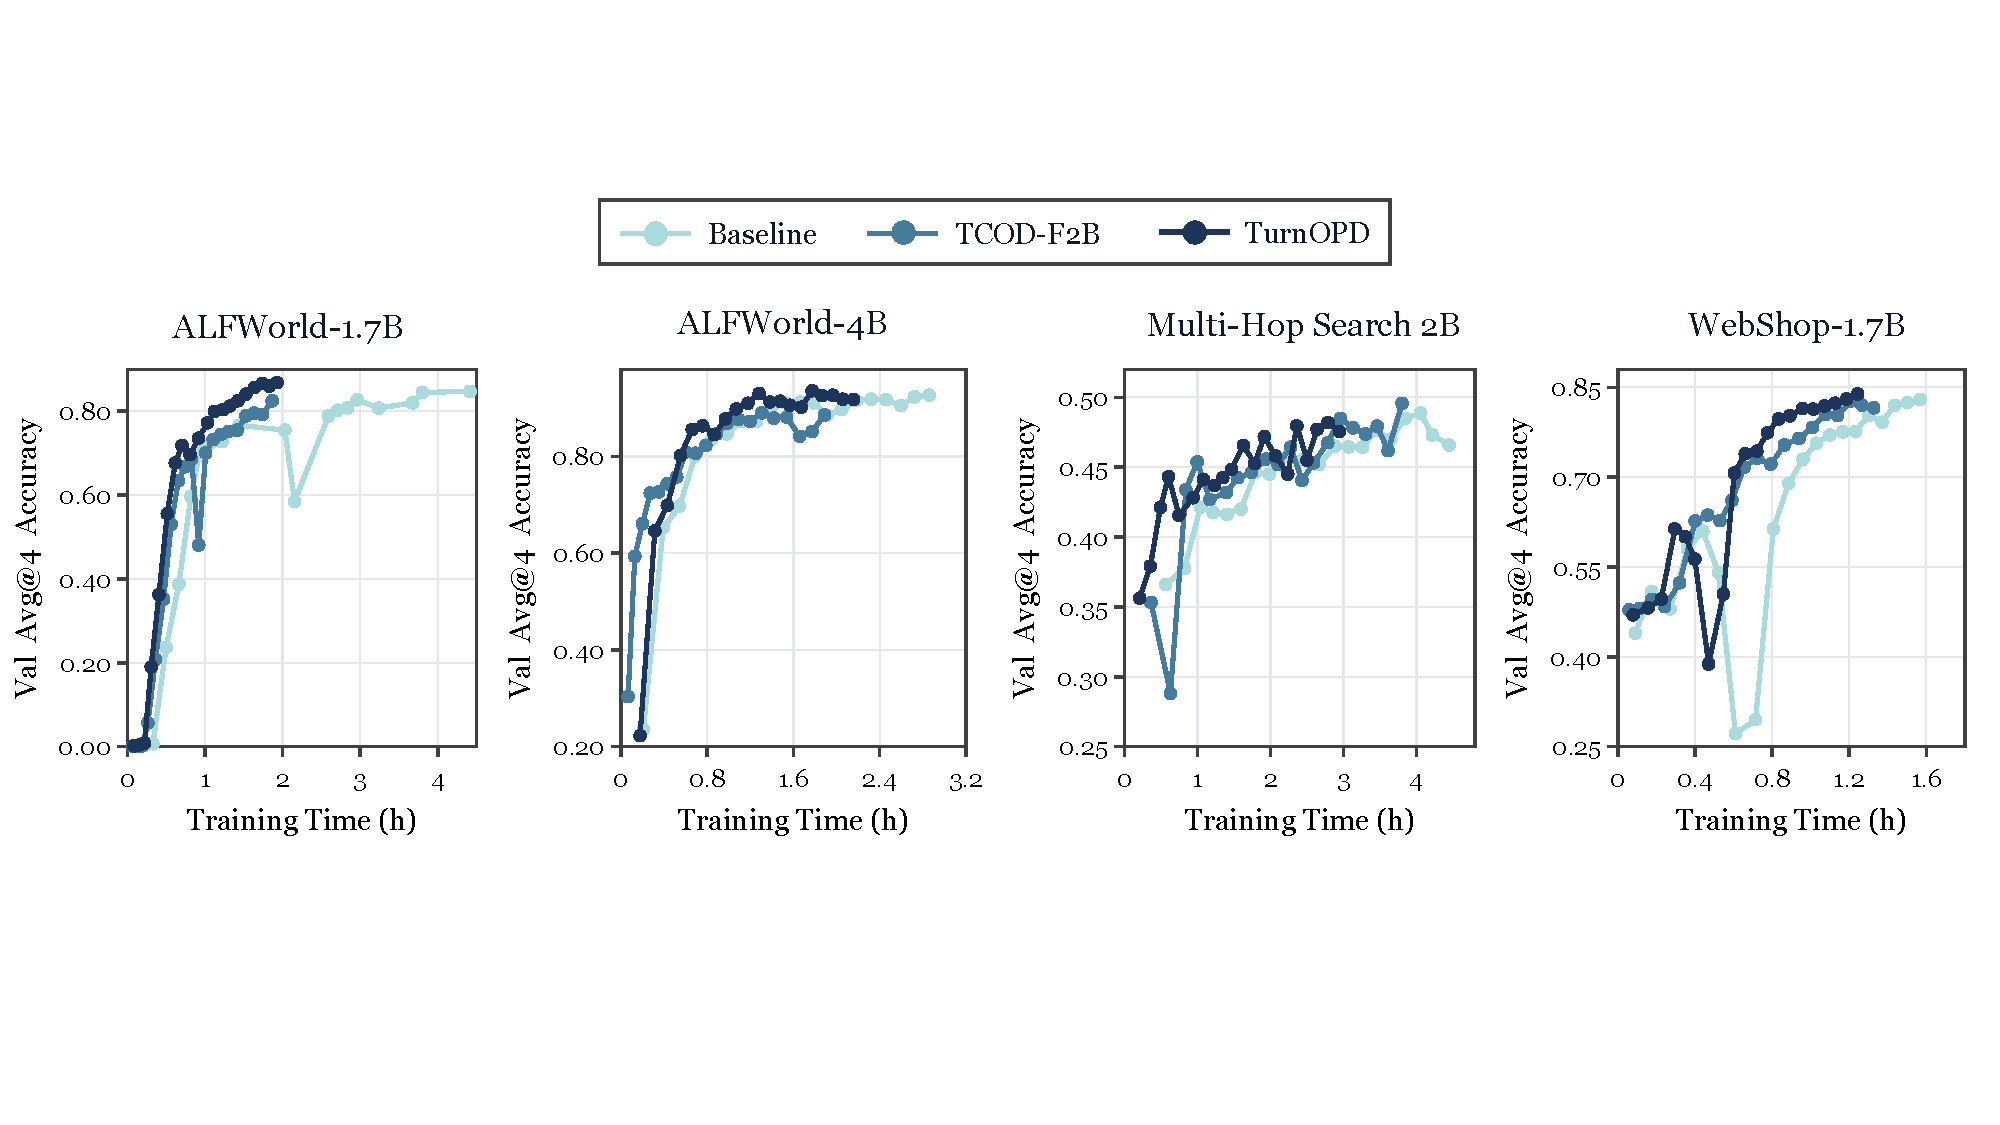
\includegraphics[width=\textwidth]{figures/iso_time_efficiency.pdf}
    \caption{Main-result iso-time efficiency.
    The x-axis is cumulative training time, computed as the running sum of
    per training step time.
    TurnOPD improves the accuracy--time frontier on each task type.}
    \label{fig:crosstask}
    \end{figure}

\begin{table*}[tbp]
    \centering
    \caption{ALFWorld category-level accuracy under the Least-Time protocol.
    Category scores report avg@4 before the same wall-clock cutoff used in
    Table~\ref{tab:main}.}
    \label{tab:alfworld-category}
    \scriptsize
    \setlength{\tabcolsep}{5pt}
    \begin{tabular}{>{\raggedright\arraybackslash}m{1.6cm}
        >{\raggedright\arraybackslash}m{1.4cm}
        >{\centering\arraybackslash}m{1.3cm}
        >{\centering\arraybackslash}m{1.3cm}
        >{\centering\arraybackslash}m{1.3cm}
        >{\centering\arraybackslash}m{1.3cm}
        >{\centering\arraybackslash}m{1.3cm}
        >{\centering\arraybackslash}m{1.3cm}
        >{\centering\arraybackslash}m{2cm}}
    \toprule
    \textbf{Student}
    & \textbf{Method}
    & \textbf{2Obj}
    & \textbf{Heat}
    & \textbf{Cool}
    & \textbf{Clean}
    & \textbf{Place}
    & \textbf{Look}
    & \makecell[c]{\textbf{Overall Avg@4}\\\textbf{Least-Time}} \\
    \midrule
    \multirow{5}{1.85cm}{\raggedright Qwen3-1.7B} & Zero-Shot & 0.00 & 0.00 & 0.00 & 0.00 & 0.00 & 0.00 & 0.00 \\
     & Teacher & 92.50 & 93.40 & 84.09 & 92.34 & 91.49 & 91.28 & 90.75 \\
     & Vanilla OPD & 76.41\avgstd{2.77} & 73.82\avgstd{2.15} & 65.45\avgstd{3.51} & 73.39\avgstd{2.57} & 75.93\avgstd{2.27} & 78.34\avgstd{2.68} & 73.52\avgstd{1.84} \\
     & TCOD-F2B & 82.66\avgstd{2.70} & 80.19\avgstd{1.20} & 74.43\avgstd{3.63} & 79.03\avgstd{0.99} & 82.18\avgstd{2.14} & 83.87\avgstd{1.76} & 80.06\avgstd{1.43} \\
     & \cellcolor{blue!9}\textbf{TurnOPD} & \cellcolor{blue!9}\textbf{87.97}\avgstd{0.27} & \cellcolor{blue!9}\textbf{85.97}\avgstd{2.09} & \cellcolor{blue!9}\textbf{80.34}\avgstd{0.38} & \cellcolor{blue!9}\textbf{84.58}\avgstd{1.55} & \cellcolor{blue!9}\textbf{87.10}\avgstd{2.67} & \cellcolor{blue!9}\textbf{89.53}\avgstd{2.06} & \cellcolor{blue!9}\textbf{85.60}\avgstd{0.95} \\
    \midrule
    \multirow{5}{1.85cm}{\raggedright Qwen3-4B} & Zero-Shot & 4.38 & 5.19 & 3.64 & 5.24 & 11.70 & 21.51 & 8.17 \\
     & Teacher & 92.50 & 93.40 & 84.09 & 92.34 & 91.49 & 91.28 & 90.75 \\
     & Vanilla OPD & 92.97\avgstd{0.52} & 89.50\avgstd{0.39} & 90.34\avgstd{2.21} & 90.02\avgstd{1.08} & \textbf{91.49}\avgstd{1.95} & 91.28\avgstd{0.92} & 90.79\avgstd{0.61} \\
     & TCOD-F2B & 88.91\avgstd{1.20} & 85.26\avgstd{2.86} & 85.00\avgstd{2.51} & 84.17\avgstd{2.29} & 87.23\avgstd{3.24} & 90.26\avgstd{1.86} & 86.50\avgstd{1.88} \\
     & \cellcolor{blue!9}\textbf{TurnOPD} & \cellcolor{blue!9}\textbf{94.53}\avgstd{2.44} & \cellcolor{blue!9}\textbf{91.04}\avgstd{1.45} & \cellcolor{blue!9}\textbf{90.68}\avgstd{0.75} & \cellcolor{blue!9}\textbf{91.94}\avgstd{2.26} & \cellcolor{blue!9}90.96\avgstd{1.36} & \cellcolor{blue!9}\textbf{91.86}\avgstd{2.36} & \cellcolor{blue!9}\textbf{91.73}\avgstd{1.41} \\
    \bottomrule
    \end{tabular}
    \vspace{-0.2cm}
\end{table*}

\begin{table*}[tbp]
    \centering
    \caption{Multi-Hop Search category-level accuracy under the Least-Time
    protocol. Category scores report avg@4 over the four held-out QA sources.}
    \label{tab:multihop-category}
    \scriptsize
    \setlength{\tabcolsep}{5pt}
    \begin{tabular}{>{\raggedright\arraybackslash}m{2.3cm}
        >{\centering\arraybackslash}m{1.5cm}
        >{\centering\arraybackslash}m{1.6cm}
        >{\centering\arraybackslash}m{1.6cm}
        >{\centering\arraybackslash}m{1.7cm}
        >{\centering\arraybackslash}m{2.2cm}}
    \toprule
    \textbf{Method}
    & \textbf{PopQA}
    & \textbf{NQ}
    & \textbf{2Wiki}
    & \textbf{HotpotQA}
    & \makecell[c]{\textbf{Overall Avg@4}\\\textbf{Least-Time}} \\
    \midrule
    Zero-Shot & 38.25 & 29.00 & 39.25 & 37.81 & 36.08 \\
    Teacher & 59.50 & 52.50 & 72.00 & 52.00 & 59.00 \\
    Vanilla OPD & 48.00\avgstd{0.31} & \textbf{40.88}\avgstd{1.07} & 50.81\avgstd{1.15} & \textbf{43.39}\avgstd{0.53} & 45.77\avgstd{0.48} \\
    TCOD-F2B & 47.81\avgstd{1.01} & 39.38\avgstd{0.38} & 53.25\avgstd{3.05} & 42.12\avgstd{1.26} & 45.64\avgstd{1.06} \\
    \cellcolor{blue!9}\textbf{TurnOPD} & \cellcolor{blue!9}\textbf{49.38}\avgstd{1.64} & \cellcolor{blue!9}40.69\avgstd{1.12} & \cellcolor{blue!9}\textbf{56.00}\avgstd{2.49} & \cellcolor{blue!9}42.89\avgstd{0.98} & \cellcolor{blue!9}\textbf{47.24}\avgstd{1.03} \\
    \bottomrule
    \end{tabular}
    \vspace{-0.2cm}
\end{table*}


\subsection{Diagnostic--Controller Alignment}
\label{sec:exp:diag}
The main results confirm that TurnOPD effectively improves both the accuracy and compute efficiency frontiers. To further validate the effectiveness of the adaptive controller, we examine whether the controller’s behavior aligns with our diagnostic metrics that motivated its design.

Figure~\ref{fig:diag-align} illustrates the dynamics of TurnOPD's rollout-depth adaptation. Specifically, we plot the survivor-weighted raw-KL centroid $\Heff$ (representing the efficiency arm) and the success-conditioned completion quantile $\Hcov$ (representing the coverage arm) as defined in Section~\ref{sec:method:A}. The controller adaptively targets the maximum of these two quantities at each step. During initial warm-up phases before sufficient successful rollouts appear, $\Hcov$ is set to zero to ensure that the observed KL centroid remains visible. Across tasks, we observe distinct controller behaviors: (1) in ALFWorld, the coverage constraint ($\Hcov$) quickly dominates once successful trajectories emerge, encouraging longer rollouts; (2) for WebShop, the controller maintains a moderate coverage lower bound throughout; and (3) in Multi-Hop Search, the balance shifts dynamically between the efficiency and coverage arms. These plots confirm the intended division of labor: $\Heff$ ensures nontrivial efficiency, while $\Hcov$ prevents the controller from selecting overly short rollouts that would limit coverage of successful completions.

\begin{figure}[htbp]
\centering
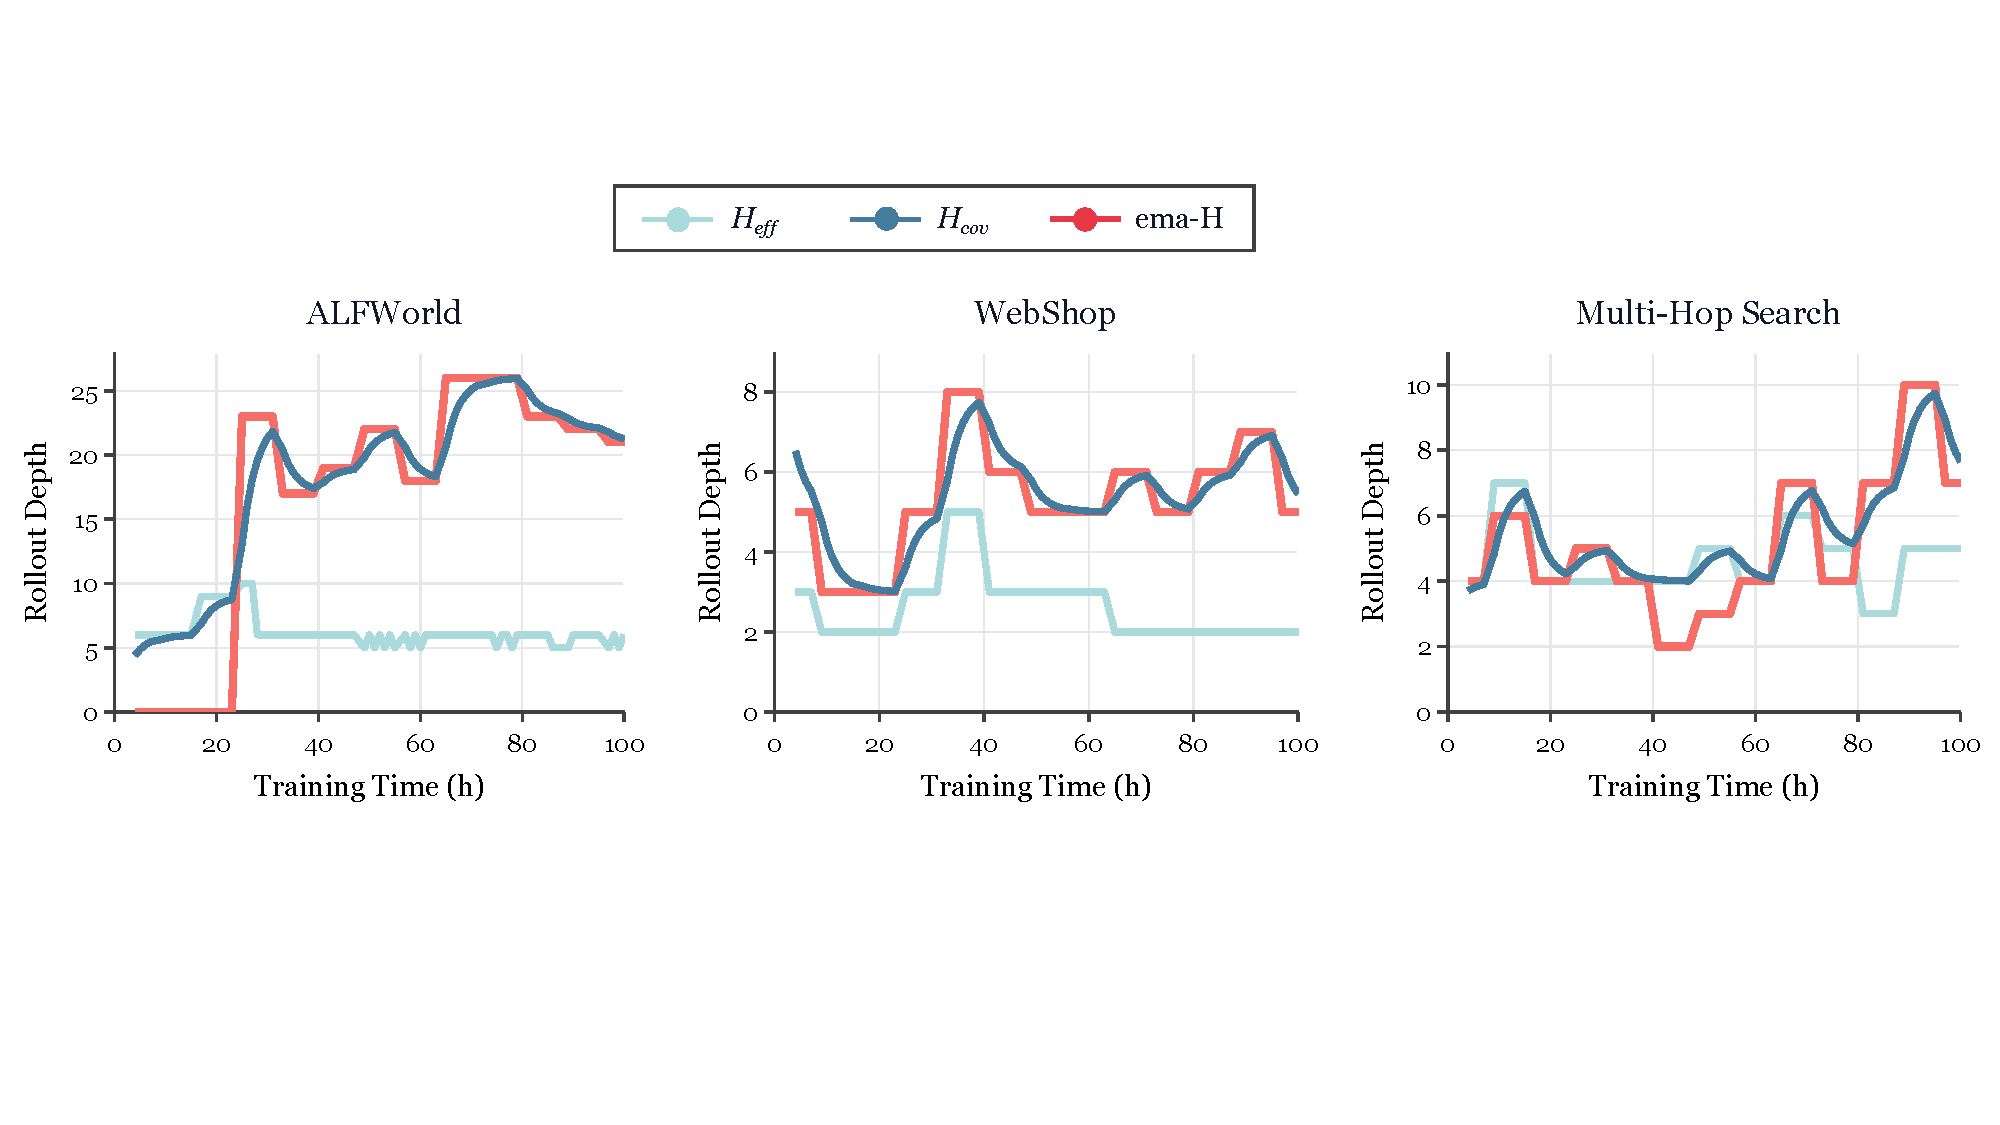
\includegraphics[width=0.9\linewidth]{figures/horizon.pdf}
\caption{Rollout-depth diagnostic replay. For each TurnOPD run, we plot the
survivor-weighted raw-KL centroid $\Heff$, the success-coverage lower bound
$\Hcov$, and the counterfactual EMA horizon $\hat H_{\mathrm{EMA}}$
obtained by replaying $\max(\Heff,\Hcov)$. Values use the 0-based turn-index
convention; the applied rollout cap is approximately
$\mathrm{round}(\hat H)+1$.}
\label{fig:diag-align}
\end{figure}
